\section{Fundamentals of Information Security}
Security is built on top of well established principles like the confidentiality, integratity and availability triad and the gold standard. This section discusses those principles as well as the role of cryptography. In addition, the software development life cycle is discussed and the technologies and languages.

\subsection{The Confidentiality, Integrity, and Availability Triad}
Security can be complicated as discussed in Section \ref{sec:challenges-in-is}. Nonetheless, as described in Table \ref{fig:cia}, the confidentiality, integrity, and availability (CIA) triad, provides a model to think about and discuss security concepts. It is commonly discussed in the information security literature \cite{andress2014the} \cite{srinivasan2016cissp} \cite{death2017information}. The CIA triad is commonly referred to as tenets of information security. Information assets that are tied to an application can be associated to a specified CIA requirement represented as a number or values suchlike, high, medium, or low, which can be determined through risk analysis \cite{srinivasan2016cissp}. 

\begin{figure}[!h]
    \centering
    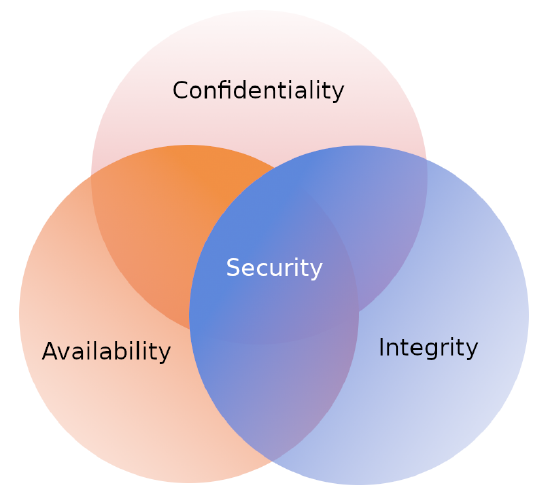
\includegraphics[width=0.5\textwidth]{../../img/chapter_2/cia-triad.png}
    \caption{The CIA Triad}\label{fig:cia}
\end{figure}

\subsubsection{Confidentiality}
Confidentiality describes the capability to secure assets from parties that do not have the authorization to view. 
\subsubsection{Integrity}
The second concept describes the ability to prevent data from being changed in an unauthorized or undesirable manner. Integrity preserves the consistency of information both internally and externally.

\subsubsection{Availability}
The final concept describes the ability to access data when required.

\subsection{The Gold Standard}

\subsubsection{Authentication}
Identification is the claim of identity by a person, process, or other entity without implying the authenticity of the claim or privileges that could be affiliated with the identity. Many methods exists to claim our identity such as name abbreviations, fingerprints, portraits, and many more.

Authentication is the procedure used to validate whether the claim of identity is correct. A real world example of authentication would be the usage of a username and password combination inside an application. Depending on the security level required of an asset, more factors can be used for the authentication mechanism, also known as multifactor authentication.

\subsubsection{Authorization}
Besides claiming an identity and confirming the validity of that claim, we need to decide what the party is allowed to do and if access to specific resources are allowed or denied. 
% This can be accomplished through the concepts: authorization and access control.

\subsubsection{Principle of least privilege}
An important authorization concept is the principle of least privilege. It mandates that only the bare minimum of access to a party should be allowed to function. As an example, a user account is only granted the access needed to perform their routine work. It is a very simple security measure that requires minimal effort, and it is highly effective.

\paragraph{Access control}
At a high level, access control is about restricting access to a resource. Access control can be divided into two groups to either improve the design of physical security or cybersecurity. Generally, four basic actions can be performed: 
\begin{itemize}
    \item allowing
    \item access
    \item denying access
    \item limiting access
    \item revoking access
\end{itemize}
Most access control issues or situations can be described through these. Moreover, users that are not authorized should not be granted access. Therefore, it is best practice to disallow access by default.

There are two main methods that can be considered to implement access controls: access control lists (ACLs) and capabilities. ACLs, often referred to as "ackles", are a very common choice of access control implementation. Typically, ACLs are implemented in the file systems on which our operating systems run and to control the flow of traffic in the networks to which our systems are connected. A capability-based approach to security uses tokens that manages our access. A good analogy would be the usage of a personal badge that grants access to certain doors inside a building. Notably, the right to access a resource is based completely on possession of the token, not who possesses it.

\subsubsection{Auditing}
After going through the process of identification, authentication, and authorization, it is important to keep track of the activities that have occurred. Despite access being granted to the party, it is important that the party behaves according to the rules as it concerns to security, ethics, business conduct, and so on. With an abundance of digital assets it has become a vital task to ensure that rules set forth are abided by.

% % \paragraph{Accountability}
% % Accountability depends on identification, authentication, and access control being present in order to trace activities and associate the transactions back to the source. Moreover, maintaining accountability ensures that organizations are in compliance with any laws or regulations associated with the type of data being handled or the industry in which the organization operates. 

% From a security perspective, accountability introduces several beneficial features. Without the information that is being monitored or logged, there would be no foundation to maintain a higher security posture.

% \paragraph{Auditing}
% A foremost approach to assure accountability through technical means is by ensuring that accurate records are registered of who did what when they did it. Without auditing there exists no ability to assess activities over a period of time. Consequently, there is no way to assist accountability on a large scale. Within the scope of information security, we primarily look at access to or from systems. Some common audited items are passwords and software licensing.

\subsection{Cryptography}
Cryptography is the science of ensuring that assets are kept secure. The foremost security measure allowing cryptography is encryption, and often the terms are used interchangeably. Although in reality, encryption is a subset of cryptography. Encryption is the transformation of plaintext into ciphertext. 

Cryptology is not a recent invention. At the very least cryptology can be traced back as far as 2500 years and was considered an obscure science. It was well established with both ancient Greeks and Romans who practiced different forms of cryptography. A classic example of ancient cryptography is the Ceasar cipher as seen in Figure \ref{fig:ceasar-cipher}. After the fall of the Roman Empire, cryptology was flourishing in the Arabic world \cite{dooley2018history}.

\begin{figure}[!h]
    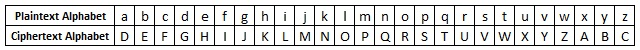
\includegraphics[width=\textwidth]{../../img/chapter_2/ceasar-cipher.jpg}
    \caption{Ceasar Cipher}\label{fig:ceasar-cipher}
\end{figure}

Without cryptography, much of the internet-based activities we benefit from today would be at great risk. In fact, cryptography is essential in computing, networking and the great set of transactions that take place over such devices in everyday life. Cryptography has permitted us to become a very network-centric society. 
Data can be protected at rest, in motion, and to a certain extent, in use, because of cryptography. Thus allowing us to securely communicate and perform transactions when sensitive data is involved.

The process of encrypting plaintext and decrypting ciphertext is described as a cryptographic algorithm. In order to either encrypt or decrypt a message, cryptographic algorithms commonly use a key, or multiple keys, with a range of possible values for the key referred to as the keyspace. The harder the keyspace, the harder it is to decrypt the message. We will take a brief look at some popular cryptographic algorithms.

\subsubsection{Symmetric cryptography}
Symmetric cryptography, also referred to as private key cryptography, utilizes a single key for both encryption of the plaintext and the decryption of the ciphertext as can be seen in Figure \ref{fig:sym-crypt}. A symmetric cipher only works if both the sender and the receiver are in possession of the same key to unlock the cipher. Therefore, everyone who uses a symmetric cipher must have the same set of keys and must use them in the correct order \cite{dooley2018history}.

% Several algorithms exists to implement symmetric key cryptography such as, AES, DE3, 3DES, RC4, Blowfish, etc. \cite{Chandra_2014}.

\subsubsection{Asymmetric cryptography}
When a different key is used for encryption and decryption, we have an asymmetric system in place. Asymmetric cryptography can also be referred to as public key cryptography. Asymmetric cryptography relies on a public key to encrypt data from the sender, and a private key to decrypt data that arrives at the receiving end as seen in Figure \ref{fig:asym-crypt}. Due to the mathematical complexity of the operations to create the private and public keys, no method exist at present to reverse the private key from the public key.

\begin{figure}
    \centering
    \begin{minipage}{.5\textwidth}
        \centering
        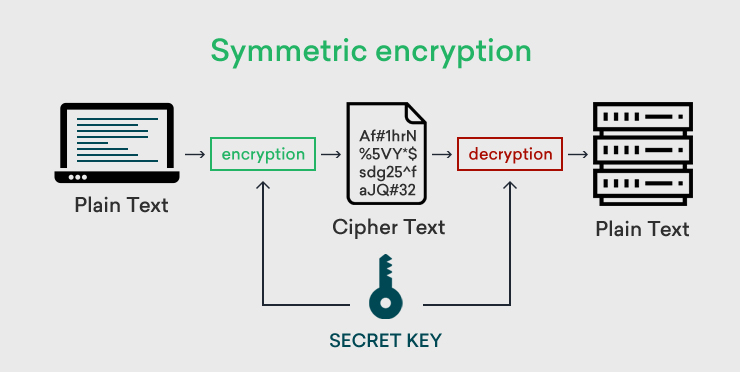
\includegraphics[width=.9\textwidth]{../../img/chapter_2/symmetric-cryptography.jpg}
        \caption{Symmetric encryption}\label{fig:sym-crypt}
    \end{minipage}%
    \begin{minipage}{.5\textwidth}
        \centering
        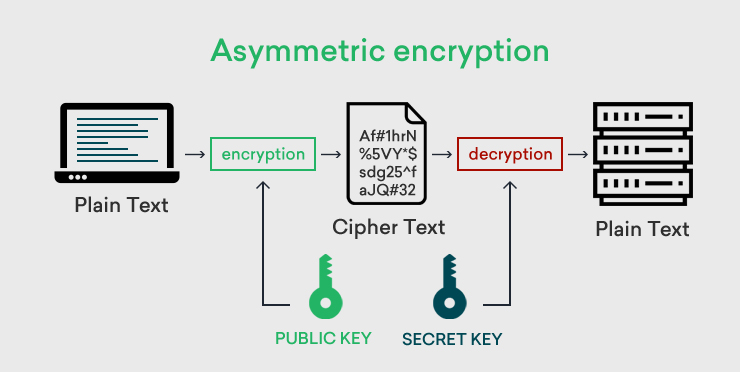
\includegraphics[width=.9\textwidth]{../../img/chapter_2/asymmetric-cryptography.jpg}
        \caption{Asymmetric encryption}\label{fig:asym-crypt}
    \end{minipage}
\end{figure}

\subsubsection{Hash functions}
Unlike both symmetric and asymmetric cryptography, which relies on keys for encryption and decryption, there are algorithms that do not require keys, known as hash functions. Hash functions generate a generally unique and fixed-length hash value, referred to as a hash, based on the original message as seen in Figure \ref{fig:hash}. Any form of change to the message will change the hash as well. Furthermore, hash functions do not allow for  contents of the message to be read, though it can be utilized to determine the confidentiality of the message. Some hash algorithms include: Message-Digest 5 (MD5), MD2, MD4, SHA-2, and RACE. 

\begin{figure}[!h]
    \centering
    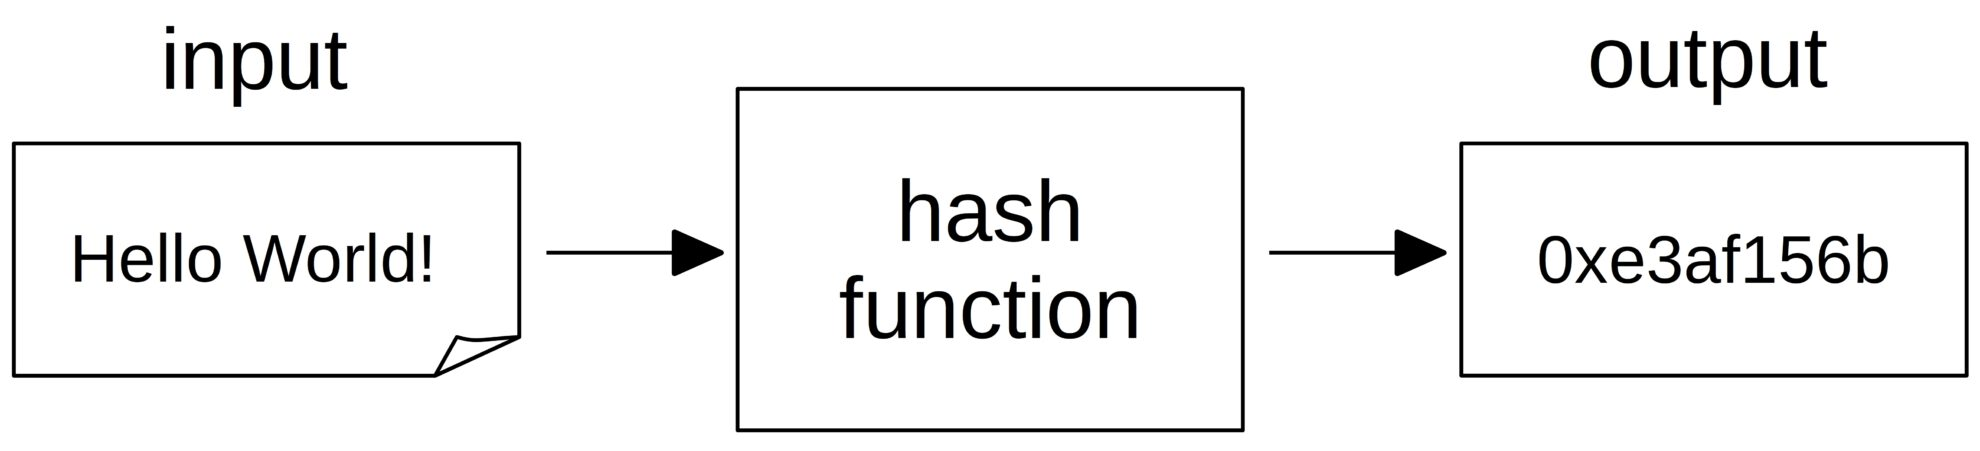
\includegraphics[width=0.5\textwidth]{../../img/chapter_2/hash-functions.jpg}
    \caption{Hash function}\label{fig:hash}
\end{figure}

\paragraph{Digital signatures}
A good example of where hash functions are utilized are digital signatures. To detect any changes to the content of the message, digital signatures make it possible to sign a message to ensure the authenticity from the sending party. This is accomplished by generating a hash of the message, and then use the senders private key to encrypt the hash, thereby creating a digital signature. The receiving party can use the sender's public key to decrypt the digital signature, thereby restoring the original hash of the message.

Digital signatures are now recognized as legally binding in many countries, allowing them to be used for certifying contracts or notarizing documents, for authentication of individuals or corporations, as well as components of more complex protocols. Broadly speaking, a digital signature is analogous to a handwritten signature, that provides much stronger security guarantees \cite{katz2010digital}. 

\subparagraph{Certificates}
Another form of cryptography for message signing, is the usage of digital certificates, commonly known as certificates. Certificates link together a public key and an individual, typically by taking the public key and something to identify the individual, suchlike a name and address, and having them signed by a certificate authority (CA). A CA is a trusted entity that is responsible for digital certificates. The advantage of using a certificate is that it provides verification that a public key actually is associated with a particular individual.
